\section{\sysname Architecture} \label{sec:hardenUI}
% Protecting User Input Integrity by Visual Supervision}

We now describe in detail how \sysname addresses the remaining challenges discussed in the previous section to ensure that all remote requests truly correspond to a legitimate user's intended input. \sysname design consists of two parts. First, the server-side requires two sets of modifications: i) in the web forms to make them suitable for UI analysis and input data extraction, and ii) a server-side program that compares the data from the host browser and the smartphone app. Second, the smartphone application captures the host display and analyze the UI, and extract input data.


\subsection{Verifying the Integrity of the User Interface}
\label{sec:systemDesign:webpage}

The precise layout of web forms is as important to protect as the user input: the adversary can alter the semantics of the input by manipulating the UI the user sees.
Sensible changes can be in values, e.g., in the form of Figure~\ref{fig:traceMatching}, changing ``USD'' to another currency to trick into entering a bigger amount, or in element position, e.g., swapping two labels or moving them to trick the user into using the wrong measurement units.
Therefore, it is crucial to assert that the interface the user sees while interacting matches the expectations of the server, both in textual values and in position of the UI elements.

We now discuss a minimal set of design guidelines that standardize the web form's aspect to harden it against such attacks.
By following these guidelines, a web form can be precisely described in a single JSON form specification file, which the \app obtains from the server, and uses as a guide during supervision of user input.
We show an example of such guidelines in Figure~\ref{fig:runningExample}, and its corresponding form specification in Listing~\ref{code:formSpecification}.


% \begin{figure}[t]
% 	\centering
% 	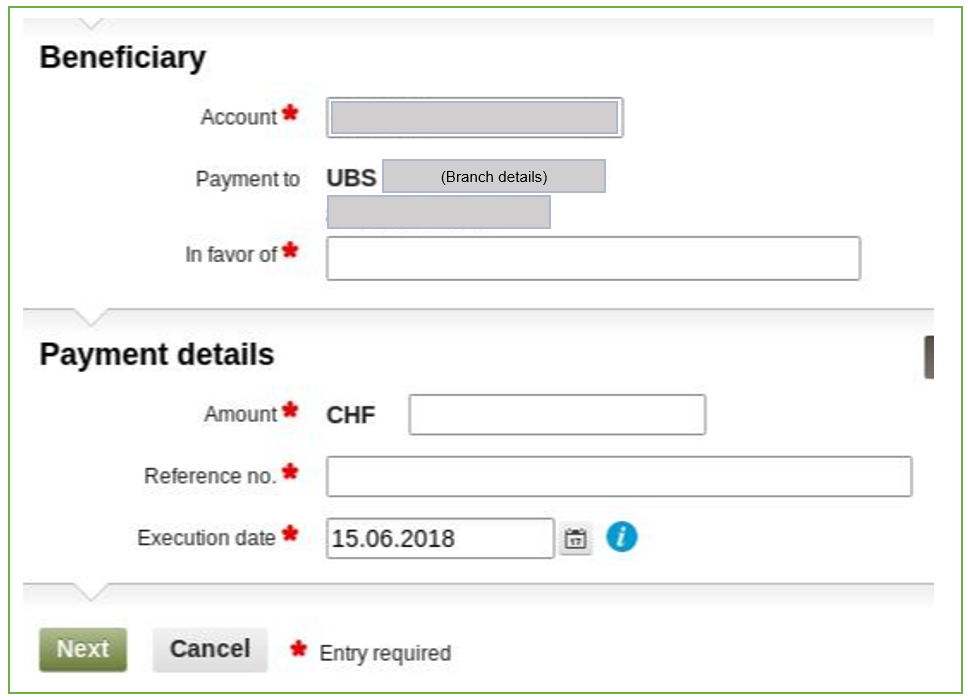
\includegraphics[width=\linewidth]{./img/formUBS.PNG}
% 	\caption{\textbf{Real-world motivation for the running example.}
% 		The design of the running form used throughout the paper and in the user study is based on the web banking interface of one of the large financial organizations.
% 	}
% 	\label{fig:formUBS}
% \end{figure}

\begin{figure}[t]
	\centering
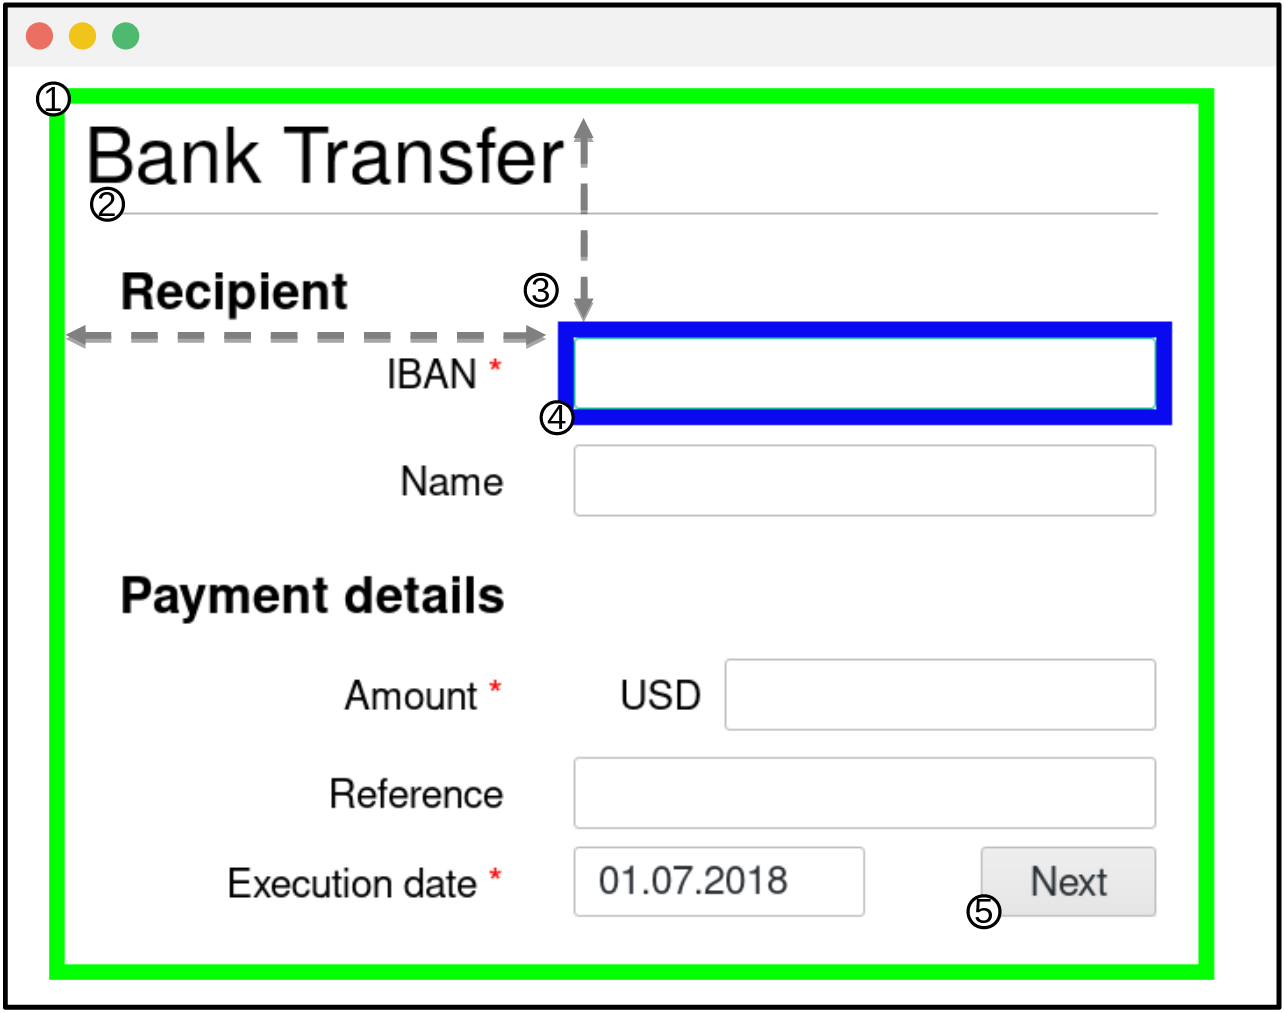
\includegraphics[width=0.55\linewidth]{chapters/IntegriScreen/img/runningExample.png}
	\caption[\name{} web form features]{\textbf{\name{} web form features:} \one form boundary, \two form identifier, \three precise positioning of elements, \four the element in focus, \five submit button.
% 		The green rectangle \one supports the form localization and perspective realignment.
% 		The form is defined by its title \two and its precise specification of each UI element's relative position \three.
% 		The currently focused element is clearly emphasized by a blue rectangle \four, and the form is submitted upon a button press \five.
% 		The interface is based on the a real-world web form used for online banking by a major organization (shown in Figure~\ref{fig:formUBS}).
}
	\label{fig:runningExample}
\end{figure}

\lstset{
	string=[s]{"}{"},
	stringstyle=\color{blue},
	comment=[s]{:}{,},
	commentstyle=\color{black},
	basicstyle=\small\ttfamily,
	caption={Form specification example corresponding to the form in Figure~\ref{fig:runningExample}.},
	label = code:formSpecification,
	firstnumber=1
}
\begin{figure}[t]
\begin{lstlisting}[mathescape=true]
    "ratio": "1280:960",
    "page_id": "Bank Transfer",
    "elements": [
    {"id": "IBAN_label",
      "type": "label",
      "initialvalue": "IBAN *",
      "x_position": 10,"y_position": 25, "width": 30, "height": 8},
    {"id": "IBAN_value",
      "type": "input",
      "initialvalue": "",
      "x_position": 42, "y_position": 25, "width": 50, "height": 8},
    (...) ]
\end{lstlisting}
\end{figure}


\begin{enumerate}
	\item[\one] \textbf{Form Border.}
	\sysname relies on the web form being surrounded by a visible boundary, which serves two roles:
	(i) helping the \app in estimating and removing the pose between the screen and the mobile device for different spatial arrangements; and
	(ii) limiting the area of visual analysis of the screen by excluding other OS/browser UI elements and thus increasing user's privacy.
	For simplicity, the current prototype uses a solid green color to indicate the form border.
	However, this can be fully customized as long as the four corners that indicate the protected area can be detected and tracked by the mobile app~\cite{zhang2002visual}.


	\item[\two] \textbf{Form Title.} \sysname requires that each form has an unique title to download its corresponding specification file.
	While in this chapter, we assume that the unique form identifier is displayed in the upper left corner, we emphasize its URL could also serve this purpose.
	As we discuss in Section~\ref{sec:securityAnalysis}, the adversary can only cause a denial-of-service by manipulating the form title.

	\item[\three] \textbf{Form Specification.}
	To enable UI verification, \sysname requires that the expected relative positions of all UI elements is known, and a specification of such positions is available to the mobile app after the client loads the web form.
	An example of such specification is given in Listing~\ref{code:formSpecification}: the borders of each UI element are precisely defined relative to the frame border, as are their type (label or input element), and initial values.
	Such specification allows the application to ensure that none of the expected UI elements are missing, modified, or added, thus preventing UI-based manipulation.

	\item[\four] \textbf{Focused Element Border.}
	The input element that is currently being edited (in focus) must be highlighted to indicate the screen area where data changes are allowed to happen.
	While such a visual guide is already implemented on most modern browsers (and we use a blue rectangle for simplicity), \sysname allows for full customization of its design.
	We mandate that while the focused element is changing the remainder of the form (outside of the focus) must remain static.
	Finally, we also restrict how quickly can the focus move away from an element whose value has changed.
	As we discuss in Section~\ref{sec:systemDesign:phone}, this does not limit normal user behavior, while at the same time ensuring stable OCR performance and detection of on-screen modification attacks.

	\item[\five] \textbf{Visible Request Data.}
	Visual supervision requires that the results of entering the sensitive data that comprises the remote request are clearly shown on the client's screen.
	This, for example, allows mouse interaction to change the state of checkboxes or a calendar widget to choose a date, as long as the chosen value is visibly shown afterwards.
	We assume that the form includes a ``Submit'' button that generates the remote request towards the server.

\end{enumerate}

The above requirements are highly extensible, as they do not enforce a specific layout and allow services that implement \name to use their own branding and style.
We further discuss relaxing or modifying some of the requirements in Section~\ref{sec:discussion}.



\subsection{Server-side Component}
\label{sec:systemDesign:webserver}

\sysname requires a server-side component that carries out the \emph{input trace matching} between i) the user input from the HTTP payload sent by the browser, and ii) signed input from the \sysname \tls payload. One such example is illustrated in Figure~\ref{fig:traceMatching}. If these two traces mismatch, the \name server-side component notifies the \name mobile app.

\iffalse
Protecting an existing remote service with \sysname requires the addition of a server component, fully owned by the remote service.
This server component ensures that only a request with a matching \POI is actually forwarded to the remote service, which can thus remain unmodified.
It provides the following functionalities:
\begin{enumerate}[leftmargin=*]
    \item \textbf{Serves} the web form specification upon request from the \name mobile app.

    \item \textbf{Receives} data from the client.

    \item \textbf{Receives} \PsOI from the mobile app.

    \item \textbf{Matches} received data with their corresponding POIs.
    If there is no mismatch, the server component forwards the client's request to the remote service, otherwise, the request is dropped.

	\item \textbf{Notifies} the client and mobile device about the outcome.


\end{enumerate}
\fi

\myparagraph{Generating specifications for web forms}
The mobile app requires that the layout of the web form is described in a specification file, which can either be provided by developers of the remote service, or automatically generated by the \sysname server component.
We note that the other direction is also possible: the server component generates the valid HTML web form based on its specification.
We implement this approach for the experimental evaluation in Section~\ref{sec:experimentalEvaluation}, in which we evaluate the performance of the system on hundreds of tests on randomly generated web forms.




\subsection{\sysname Smartphone Application} \label{sec:systemDesign:phone}

The mobile device application provides an independent, out-of-band confirmation of user's intended input despite the client compromise.
This is achieved by verifying that the user interface matches its specification during user interaction, supervising against any on-screen modification attacks, and capturing the data shown on the client's screen to generate and send a respective \POI.

After being loaded by the user, the \sysname mobile app performs the following steps:
\begin{enumerate}%[leftmargin=*]
    \item \textbf{Locates} the border of the web form shown on the client's display, realigns the captured video feed to a flat perspective, and extracts the form's unique title.
    \item \textbf{Loads} the corresponding UI specification file from the server.
    \item \textbf{Continuously verifies that the UI} of the web form shown on the client device matches its specification, i.e., that all UI elements are present and that none have been modified or added.
    \item \textbf{Continuously supervises user input}, allowing only the element in focus to change, only when the user is present and active.
	\item \textbf{Submits} the generated \POI to the server.
    \item \textbf{Notifies} the user about the result of server's data comparison: either success (if client and \md -submitted data match) or failure (in case of data mismatch).
    In the latter case, the user is allowed to confirm which of the two versions of submitted data he wants to use (or a combination thereof).
    For additional security guarantees, the user confirms her choice in a hardware protected user interface which is available since Android 9~\cite{androidConfirmation}.
\end{enumerate}

Steps \textbf{(3)} and \textbf{(4)} form the core of the \name mobile app, as they are continuously executed for each frame that the mobile device captures to protect input integrity -- we now describe them in more detail.


\myparagraph{(3) Continuous UI Verification}
For each captured frame, the application verifies that all UI elements conform in position and text values to the expectation.
Labels are never allowed to change, thus always need to match the specification.
Input elements change as a result of user input: when they are modified, the application tracks the latest value input by the user, and verifies that it stays the same afterwards.
Finally, to detect if any UI element has been added by the adversary (which could misguide the user), the application performs text detection on the parts of the frame which should not contain any UI element according to the specification.

In the case of any missing, modified or added UI element, the application warns the user of the potential attack, both visually and by ringing or vibrating.
The application clearly augments its preview of the screen to show which elements are problematic (showing them in red), and prevents any data input until the mismatch is solved.



\myparagraph{(4) Continuous Input Supervision}
Besides the layout of the UI, the application also supervises any change on the form to make sure it is a result of intended user interaction:

\begin{enumerate} [label=(\alph*), leftmargin=*]
    \item \textbf{Only the element in focus can change.}
    All other elements must remain the same.
    \item \textbf{Activity detection.}
    If the value of the active element changes, the app must also assure that the user is present. One way to achieve that in our scenario is to detect users hands from the camera feed.
    \item \textbf{Focus changes slowly.}
    If some active element's value changes, the focus should not change to another element in less than $x$~ms after the last edit and in less than $y$~ms since this element first came into focus.
    The server can optionally set the values of $x$ and $y$ in the specification file, otherwise default values are used (in our prototype we set $x=300$~ms and $y=2000$~ms).


\end{enumerate}


Point \textbf{(a)} ensures that the user needs to only pay attention to the value of the currently active element (which they are editing), while all other elements are \emph{protected}.
Point \textbf{(b)} ensures that no element can change while the user is not present and editing the form.
Finally, point \textbf{(c)} serves two goals: (i) ensures that any change can be correctly detected, given frame rate limitations of the mobile app; and (ii) ensures that the adversary can not quickly move the focus to another element and change its value without the user noticing, as this would either last for a minimum of several seconds, or be detected as an attack attempt.


Furthermore, to prevent the adversary from prematurely submitting the form, the \POI is submitted to the server only after the user explicitly presses the \emph{Submit} button on the mobile device.


\myparagraph{Occlusion and multi-page forms}
Our system design natively supports user interactions in which the form is temporarily occluded (e.g., changing browser tab, minimizing the browser window).
In such cases, UI verification temporarily fails, but will be repeated as soon as the form is again displayed on the client's screen: if the values of all elements are unchanged, user input is allowed again.

Such design also supports multi-page interfaces, as the application will simply store the values of all input elements on each page as the user edits them in arbitrary order.
Clearly, changes to hidden elements are not allowed, and the value is verified every time the element is displayed again (similarly to occlusions).

